\documentclass{beamer}
\mode<presentation>
\usepackage{amsmath}
\usepackage{amssymb}
%\usepackage{advdate}
\usepackage{adjustbox}
\usepackage{subcaption}
\usepackage{enumitem}
\usepackage{multicol}
\usepackage{mathtools}
\usepackage{listings}
\usepackage{url}
\def\UrlBreaks{\do\/\do-}
\usetheme{metropolis}
%\usecolortheme{lily}
\setbeamertemplate{footline}
{
	\leavevmode%
	\hbox{%
		\begin{beamercolorbox}[wd=\paperwidth,ht=2.25ex,dp=1ex,right]{author in head/foot}%
			\insertframenumber{} / \inserttotalframenumber\hspace*{2ex} 
		\end{beamercolorbox}}%
		\vskip0pt%
	}
	\setbeamertemplate{navigation symbols}{}

	\providecommand{\nCr}[2]{\,^{#1}C_{#2}} % nCr
	\providecommand{\nPr}[2]{\,^{#1}P_{#2}} % nPr
	\providecommand{\mbf}{\mathbf}
	\providecommand{\pr}[1]{\ensuremath{\Pr\left(#1\right)}}
	\providecommand{\qfunc}[1]{\ensuremath{Q\left(#1\right)}}
	\providecommand{\sbrak}[1]{\ensuremath{{}\left[#1\right]}}
	\providecommand{\lsbrak}[1]{\ensuremath{{}\left[#1\right.}}
	\providecommand{\rsbrak}[1]{\ensuremath{{}\left.#1\right]}}
	\providecommand{\brak}[1]{\ensuremath{\left(#1\right)}}
	\providecommand{\lbrak}[1]{\ensuremath{\left(#1\right.}}
	\providecommand{\rbrak}[1]{\ensuremath{\left.#1\right)}}
	\providecommand{\cbrak}[1]{\ensuremath{\left\{#1\right\}}}
	\providecommand{\lcbrak}[1]{\ensuremath{\left\{#1\right.}}
	\providecommand{\rcbrak}[1]{\ensuremath{\left.#1\right\}}}
	\theoremstyle{remark}
	\newtheorem{rem}{Remark}
	\newcommand{\sgn}{\mathop{\mathrm{sgn}}}
	\providecommand{\abs}[1]{\left\vert#1\right\vert}
	\providecommand{\res}[1]{\Res\displaylimits_{#1}} 
	\providecommand{\norm}[1]{\lVert#1\rVert}
	\providecommand{\mtx}[1]{\mathbf{#1}}
	\providecommand{\mean}[1]{E\left[ #1 \right]}
	\providecommand{\fourier}{\overset{\mathcal{F}}{ \rightleftharpoons}}
	%\providecommand{\hilbert}{\overset{\mathcal{H}}{ \rightleftharpoons}}
	\providecommand{\system}{\overset{\mathcal{H}}{ \longleftrightarrow}}
	%\newcommand{\solution}[2]{\textbf{Solution:}{#1}}
	%\newcommand{\solution}{\noindent \textbf{Solution: }}
	\providecommand{\dec}[2]{\ensuremath{\overset{#1}{\underset{#2}{\gtrless}}}}
	\newcommand{\myvec}[1]{\ensuremath{\begin{pmatrix}#1\end{pmatrix}}}
		\let\vec\mathbf

		\lstset{
			%language=C,
			frame=single, 
			breaklines=true,
			columns=fullflexible
		}

		\numberwithin{equation}{section}

		\title{NCERT Presentation}
		\author{Arjun Pavanje,\\ EE24BTECH11005,\\IIT Hyderabad.\\}

		\date{\today} 
		\begin{document}

		\begin{frame}
			\titlepage
		\end{frame}

		\section*{Table of Contents}
		\begin{frame}
			\tableofcontents
		\end{frame}
		\section{Problem}
		\begin{frame}
			\frametitle{Problem Statement}
Solve the differential equation $y^{\prime}+y=e^x$ with initial conditions $y\brak{0}=1$      		\end{frame}
		\section{Solution}
		\subsection{Theoretical Solution}
		\begin{frame}
      \frametitle{Theoretical Solution}
Given equation is a linear first order differential equation, so laplace transform may be used to solve it. Some properties of laplace transform used are,
\begin{align}
  \mathcal{L}\brak{f\brak{t}} &= \int_0^{\infty} e^{-st} f\brak{t} \, dt\\
 \mathcal{L}\brak{\kappa f\brak{t}} &= \kappa \mathcal{L}\brak{f\brak{t}}\\
  \mathcal{L}\brak{y^{\prime}} &= sY\brak{S} - y_0
\end{align}
Where $\mathcal{L}\brak{y} = Y\brak{s}$
    \end{frame}
    \begin{frame}
Applying Laplace Transform to given differential Equation,
      {\small
\begin{align}
  \mathcal{L}\brak{y^{\prime}} + \mathcal{L}\brak{y} &= \mathcal{L}\brak{e^{x}}\\
  sY\brak{s} - y_0 + Y\brak{S} &= \int_0^{\infty} e^{-x\brak{x - 1} } dx = \frac{1}{s-1}\\
  Y\brak{s} &= \brak{\frac{y_0 - 0.5}{s+1}} + \frac{1}{2}\brak{\frac{1}{s-1}}
 \end{align}    
      }
Taking Laplace Inverse on both sides we get,
      {\small
 \begin{align}
   y &= \mathcal{L}^{-1}\brak{\frac{y_0 - 0.5}{s+1}} + \mathcal{L}^{-1}\frac{1}{2}\brak{\frac{1}{s-1}}\\
   y &= \brak{y_0 - 0.5}e^{-x} + \frac{1}{2} e^{x}
 \end{align}
    }
 Putting in $y_0 = 1$ we get,
 \begin{align}
   y = \frac{\brak{e^{x} + e^{-x}}}{2}
 \end{align}    \end{frame}
    \subsection{Computational Solution 1}
		\begin{frame}
			\frametitle{Computational Solution 1}
Solving given differential equation using bilinear transform.
Taking Laplace transform to both sides of the Differential Equation,

\begin{align}
  sY\brak{s} - y_0 + Y\brak{s} = \int_0^{\infty} e^{-x\brak{x - 1} } dx = \frac{1}{s-1}\\
  Y\brak{s} = \frac{y_0}{s+1} + \frac{1}{\brak{s + 1} \brak{s - 1}}\\
  Y\brak{s} = \brak{\frac{y_0 - 0.5}{s+1}} + \frac{1}{2}\brak{\frac{1}{s-1}}
\end{align}

Applying Bilinear Transform with $T=h$. To go from the domain of Laplace transform to that of Z-transform, we transform our $s$. On substituting we get,
    \end{frame}
		\begin{frame}
      \frametitle{Computational solution 1}
      {\small
\begin{align}
  Y\brak{s} &= \brak{y_0 - 0.5}\brak{\frac{h\brak{1 + z^{-1}} }{ \brak{2+h} + z^{-1}\brak{h-2} } } +\frac{1}{2}\brak{\frac{h\brak{1 + z^{-1}} }{ \brak{2-h} + z^{-1}\brak{2+h} } }\\
  &= \brak{\frac{y_0 - 0.5}{2+h}} \brak{\frac{h\brak{1 + z^{-1}}}{1 - \alpha z^{-1}} } + \brak{\frac{h}{2\brak{2-h}}}\brak{\frac{h\brak{1+z^{-1}}}{1 - \alpha^{-1}z^{-1}}}
\end{align}
      }
Where $\alpha = \frac{2-h}{2+h}$ \newline
Radius of convergence of the first term is, $\abs{z} > \abs{\alpha}$, for the second term it is, $\abs{z} > \abs{\alpha^{-1}}$. R.O.C of the total equation turns out to be, $\abs{z} > max \brak{\abs{\alpha}, \abs{\frac{1}{\alpha}}}$\newline
Taking $\brak{1 - \alpha z^{-1]}}$ to $R.H.S$ we get,
      {\tiny
\begin{align}
  Y\brak{s}\brak{1 - \alpha z^{-1}} = h\brak{\frac{y_0 - 0.5}{2+h}}\brak{\brak{1 + z^{-1}} } + \brak{\frac{h}{2\brak{2-h}}}\brak{\frac{h\brak{1+z^{-1}} \brak{1 - \alpha z^{-1}} }{1 - \alpha^{-1}z^{-1}}}
\end{align}
      }
    \end{frame}
		\begin{frame}
			\frametitle{Computational Solution 1}
After applying algebraic manipulations on the second term, above equation comes out to be, 
      {\small
\begin{align}
  Y\brak{s}\brak{1 - \alpha z^{-1}} &= h\brak{ \frac{y_0 - 0.5}{2+h}}\brak{\brak{1 + z^{-1}} } + \\
  &\brak{\frac{h}{2\brak{2+h}}} \brak{ \frac{1 + \alpha - \alpha^2 - \alpha^3}{1 - \alpha^{-1}z^{-1}} + \alpha^2 z^{-1} - \alpha \brak{1 - \alpha - \alpha^2} } 
\end{align}
      }
Applying inverse Z-transform,
      {\small
\begin{align}
  y_{n+1} &= \alpha y_n + h\brak{ \frac{y_0 - 0.5}{2+h}}\brak{\delta \sbrak{n} + \delta \sbrak{n-1}}+ \brak{\frac{h}{2\brak{2+h}}} \times \\
  &\brak{\brak{1 + \alpha - \alpha^2 - \alpha^3}\alpha^{-n} u \brak{n} + \alpha^2 \delta \sbrak{n-1}- \alpha \brak{1 - \alpha - \alpha^2} \delta \sbrak{n} }
\end{align}
    }\end{frame}
		\begin{frame}[fragile]
			\frametitle{Computational Solution 1}

here, $\delta$ is defined as,
      {\small
      \begin{align}
  \delta \sbrak{n-n_0} = \begin{cases}
      1 & n = n_0 \\
      0 & n \ne n_0
  \end{cases}
\end{align}
      }
Final General Difference Equation comes out to be, 
      {\small
\begin{align}
  y_{n+1} &= \alpha y_n + h\brak{ \frac{y_0 - 0.5}{2+h}}\brak{\delta \sbrak{n} + \delta \sbrak{n-1}}+ \brak{\frac{h}{2\brak{2+h}}} \times \\
  &\brak{\brak{1 + \alpha - \alpha^2 - \alpha^3}\alpha^{-n} u \brak{n} + \alpha^2 \delta \sbrak{n-1}- \alpha \brak{1 - \alpha - \alpha^2} \delta \sbrak{n} }
\end{align}
      }
		\end{frame}
    \subsection{Computational Solution 2}
		\begin{frame}[fragile]
			\frametitle{Computational Solution 2}
Finding the difference equation using trapezoid law,

Given Differential Equation,
      {\small
\begin{align}
  y^{\prime} &= -y + e^x \\
  \int_{y_n}^{y_{n+1}} dy &= -\int_{x_n}^{x_{n+1}} ydx +\int_{x_n}^{x_{n+1}} e^x dx  
\end{align}
      }
Discretizing steps using trapezoid rule, 
      {\small
\begin{align}
  y_{n+1} = y_n - \frac{h}{2}\brak{y_n + y_{n+1}} + e^{x_n}(e^h-1)
\end{align}
\begin{align}
  y_{n+1} - y_n &= -\frac{h}{2}\brak{y_n + y_{n+1}} + e^{x_n}\brak{e^h-1}\\
  y_{n+1} &= y_n\brak{\frac{2-h}{2+h}} + \frac{2e^{x_n}}{2+h}\brak{e^h-1}
\end{align}	
      }
    \end{frame}
		\begin{frame}[fragile]
			\frametitle{Computational Solution}
			\begin{figure}[h!]
				\centering
				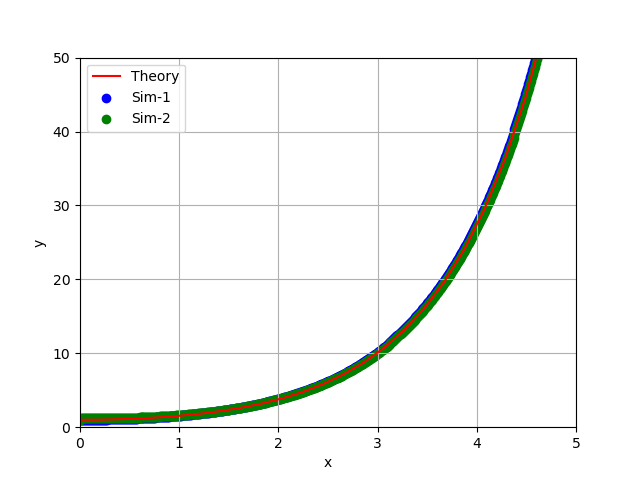
\includegraphics[width=1\columnwidth]{figs/fig.png}
				\label{stemplot}
			\end{figure}
	\end{frame}
	\end{document}
